\documentclass[twocolumn,nofootinbib]{revtex4}
%\usepackage{amsmath}
%\usepackage{iopams}
\usepackage{amsmath}
\usepackage{hyperref}
\usepackage{amssymb}
\usepackage{color}
\usepackage{epsfig}
\usepackage{latexsym}
\usepackage{tensor}
%\usepackage{wasysym}
\usepackage{comment}
%\usepackage{graphicx}
%\usepackage{psfrag}


\newcommand{\gw}{gravitational wave }
\newcommand{\gws}{gravitational waves }
\newcommand{\subgw}{_{\textrm{\scriptsize{GW}}}}
\newcommand{\ee}[1]{\!\times\!10^{#1}}
\newcommand{\prob}{{\rm Pr}}
\newcommand{\grbrate}{{{\mathcal R}_{\mathrm{grb}}}}
\newcommand{\cbcrate}{{{\mathcal R}}}
\newcommand{\diff}{{\mathrm d}}
\newcommand{\rhostar}{{\rho^*}}

\begin{document}

\title{Constraints On Short, Hard Gamma-Ray Burst Beaming Angles From
Gravitational Wave Observations}
\author{James Clark, Ik Siong Heng, Martin Hendry}
\date{\today}

\begin{abstract}
Apologies in advance for inconsistent conditioning statements in probabilities
\dots
\end{abstract}

\maketitle

\section{Introduction}

It is common in the literature to draw inferences on the rate of binary
coalescence $\cbcrate$, given some estimate for the beaming angle $\theta$ and
the observed rate of sGRBs $\grbrate$.  In this work, we investigate what
statements can \emph{currently} be made on the beaming angle itself using the
upper limits placed on $\cbcrate$ from all-sky, all-time \gw searches and
explore the potential for direct inference of sGRB  beaming angles in the
advanced detector era.

%\section{Limits On sGRB Beaming Angles From Past Gravitational Wave Searches}
\section{Inferring The sGRB Beaming Angle From Rate Measurements}
Assuming that at least some fraction of sGRBs are due to compact binary
coalescence, the observed rate of sGRBs may be written,
%
\begin{equation}\label{eq:rate2angle}
\grbrate=\epsilon\cbcrate(1-\cos \theta),
\end{equation}
%
where $\cbcrate$ is the rate of binary coalescence, $\theta$ is the beaming
angle of the outflow from the GRB and $\epsilon$ is the (generally unknown)
probability that a binary coalescence results in an observed sGRB.  In this
work, we assume
$\grbrate=10$\,Gpc$^{-3}$\,yr$^{-1}$~\cite{nakar-2007,Dietz11}.
 
Inferences of the GRB beaming angle are made from the posterior probability
density on the beaming angle $p(\theta|D,I)$.  Our goal then, is to transform
the measured posterior probability density on the rate $\cbcrate$ to a posterior
on the beaming angle.
%
First, note that the PDF $p(\theta|D,I)$ may be written as a marginalisation
over $\epsilon$ in the the joint PDF $p(\theta, \epsilon|D,I)$:
%
\begin{equation}
p(\theta) = \int_{\epsilon} p(\theta,\epsilon)~\diff \epsilon,
\end{equation}
%
where we have dropped the conditioning statements temporarily for notational
convenience.  Next, we note that the joint probability $p(\theta,\cbcrate)$ can
be written in terms of $\epsilon$ and $\cbcrate$ according to,
%
\begin{equation}
p(\theta,\epsilon) = p(\cbcrate,\epsilon)
\left\lvert\left\lvert
\frac{\partial(\cbcrate,\epsilon)}{\partial(\theta,\epsilon)}
\right\rvert\right\rvert,
\end{equation}
%
where the Jacobian matrix is given by,
% Increase matrix line spacing
\begingroup
\renewcommand*{\arraystretch}{1.5}

% matrix:
\begin{equation}
\frac{\partial (\cbcrate,\epsilon)}{\partial(\theta,\epsilon)} =
\begin{bmatrix}
\frac{\partial \cbcrate}{\partial \theta} & \frac{\partial \cbcrate}{\partial \epsilon} \\
\frac{\partial \epsilon}{\partial \theta} & \frac{\partial \epsilon}{\partial \epsilon}
\end{bmatrix}.
\end{equation}

% end line spacing increase
\endgroup
%%
Bringing all of these terms together then, and writing out the Jacobian matrix
determinant, we have
%
\begin{equation}\label{eq:marginaltheta}
p(\theta) = \frac{2\grbrate \sin
\theta}{(\cos\theta-1)^2}\int_{\epsilon} \frac{p(\epsilon)p(\cbcrate)}{\epsilon} ~\diff
\epsilon,
\end{equation}
%
where we have assumed $\epsilon$ and $\cbcrate$ are logically independent such
that,
\begin{equation}
p(\epsilon,\cbcrate) = p(\epsilon|\cbcrate)p(\cbcrate) = p(\epsilon)p(\cbcrate).
\end{equation}
%
%
To find the target PDF $p(\theta|D,I)$ then, we require the measured coalescence
rate posterior $p(\cbcrate|D,I)$, and we must specify a prior PDF for $\epsilon$
which encapsulates assumptions made about the relative rates of compact binary
mergers and sGRBs.
 
Following~\cite{Biswas09,BradyFairhurst08}, the posterior on the binary
coalescence rate may be determined from the loudest event in the \gw
analysis.  Specifically, for a foreground event rate due to  binary coalescence
$\cbcrate$, the probability of obtaning no events with ranking statistic $\rho$
greater than the observed loudested event $\rhostar$ is,
%
\begin{equation}
P_F(\rhostar | \cbcrate, C_L, T) = e^{-\cbcrate C_L(\rhostar) T},
\end{equation}
%
where $C_L(\rhostar)$ is the total luminosity to which the search is sensitive
and $T$ is the duration of the search.  The overall probability of obtaining
no events with ranking statistic $\rho>\rhostar$ is the product of obtaining
no such events from foreground \emph{and} the probability of obtaining no such
events from the background in the detector, denoted $P_B(\rhostar)$,
%
\begin{equation}
P(\rhostar|\cbcrate,I) = P_B(\rhostar|I)e^{-\cbcrate C_L(\rhostar) T}
\end{equation}
%
Using a uniform prior on $\cbcrate$ and inverting the overall probability with
Bayes' theorem, we arrive at,
%
\begin{equation}\label{eq:loudestEventPosterior}
p(\cbcrate | C_L({\rhostar}, T, \Lambda) \propto p(\cbcrate) \left[ \frac{1+\Lambda
C_L(\rhostar) T}{1+\Lambda}\right] e^{-\cbcrate C_L(\rhostar) T}
\end{equation}
%
where $p(\cbcrate)$ is the prior probability distribution on the rate.  The
quantity $\hat{\Lambda}$ measures the relative probability of detecting an event
with ranking statistic $x$ due to \gws versus the probability of an equally loud
event arising in the background distribution.  The reader is directed to
section\,3 of~\cite{BradyFairhurst08} for a full discussion of this quantity.

%
%\subsection{Incomplete Sky-Coverage \& Unknown GRB Rate}
%Marginalise over some stuff for the case of an `impure' GRB sample (unknown
%fraction of CBCs).
%\\

\section{Beaming Angle Limits From Past GW Searches}

In this section, we focus attention on the interpretation of rate upper limits
from past \gw analyses.  We first reconstruct the measured posterior on the
binary coalescence rate and go on to compute the posterior and upper limit on
the sGRB beaming angle under a range of assumptions regarding the sGRB
efficiency $\epsilon$.

The upper limit on the binary coalescence rate at confidence $\alpha$ is found
by integrating the rate posterior from zero to $\alpha$.  Assuming a uniform
prior on the rate $\cbcrate$ and using the rate posterior given by
equation~\ref{eq:loudestEventPosterior}, the upper limit on the rate
$\cbcrate_{\alpha}$ is given by equation 21 in~\cite{BradyFairhurst08}:
%
\begin{equation}
1-\alpha =  e^{-\cbcrate_{\alpha} C_L(\rhostar)T)}
\left[ 
1+ \left(\frac{\Lambda}{1+\Lambda}\right) \cbcrate_{\alpha} T C_L(\rhostar)
\right ].
\label{eq:rateIntegral}
\end{equation}
%
In the event that no \gw signal has been observed and the loudest event is
umabiguously due to background noise fluctuations, we are in the limit in which
$\Lambda \rightarrow 0$.  In this case, we simply have,
\begin{equation}
C_L(\rhostar)T = -\frac{\log(1-\alpha)}{\cbcrate_{\alpha}},
\end{equation}
%
and the value of $\cbcrate$ can be taken straight from the literature\footnote{Note
that this procedure necessarily confines our jet angle inferences based on
progenitor systems for which the rate upper limits are available.  Given that
the binary coalesence rate limits are quoted for canonical binary neutron star
and neutron star-black hole systems, both plausible sGRB progenitors, this
simply means our inferences on the jet angle are specific to each system and
treated separately.}

Using the most stringent 90\% confidence upper limit from \gw observations on
the rate of binary neutron star coalescences to date, $\cbcrate^{90\%}_{{\rm
bns}} = 1.3\times 10^{-4}$\,Mpc$^{-3}$yr$^{-1}$~\cite{S6lowmass}, gives
$C_L(\rhostar)T=17712$.  Similarly, for NS-BH systems,  $\cbcrate^{90\%}_{{\rm
nsbh}} = 3.1\times 10^{-5}$\,Mpc$^{-3}$yr$^{-1}$ gives $C_L(\rhostar)T=74277$.
The posteriors on the rates, assuming these values and $\Lambda=0$, are shown in
figure~\ref{fig:reconstructedRatePosterior}.  

\begin{figure}
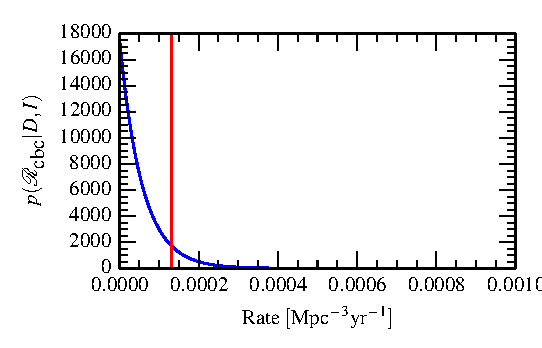
\includegraphics{rate_posterior_s6UL_TEST_deltaEffPrior-1.0.eps}
\caption{Rate posterior for S6/VSR2,3 Low-mass Search For Compact Binary
Coalescence.\label{fig:reconstructedRatePosterior}}
\end{figure}

\subsection{Known GRB Efficiency, $\epsilon$}

Figure~\ref{fig:jetPosterior} shows the resulting posterior on the GRB
beaming angle, using the transformation in equation~\ref{eq:rate2angleProb} and
our results so far.  
%
Now, the quantity of interest is the upper limit on the jet
angle~$\theta^{90\%}$:
%
\begin{equation}
0.9 = \int_{\theta^{90\%}}^{\infty}p(\theta | \cbcrate^{90\%})~\diff \theta
\end{equation}
%
This is indicated with the vertical red line in figure~\ref{fig:jetPosterior}.
We find $\theta^{90\%}=3.3^{\circ}$.


\begin{figure}
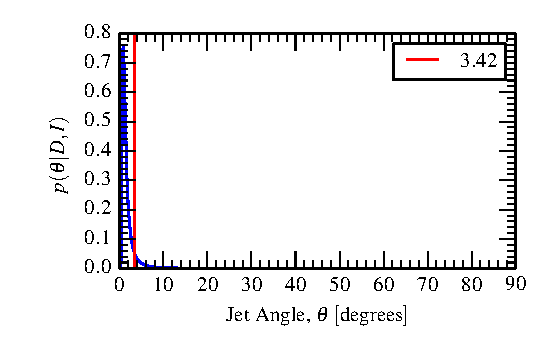
\includegraphics{jet_angle_posterior_s6UL_TEST_deltaEffPrior-1.0.eps}
\caption{Jet angle posterior derived from S6/VSR2,3 Low-mass Search For Compact Binary
Coalescence posterior / upper limit on compact binary coalescence
rate, assuming \emph{all} BNS result in sGRBs.\label{fig:jetPosterior}}
\end{figure}


\subsection{Unknown GRB Efficiency, $\epsilon$}


\subsection{Astrophysical Interpretation \& Comparison With Other Limits}
The comparison with other limits is straightforward.  I think it looks pretty
consistent with Dietz, Holtz etc (but should double check).

More importantly, however,  we've demonstrated how to get a limit on the beaming
angle.  That's all well and good but we need some astrophysical interpretation,
really.  The most obvious thing (to James) is that the beaming angle is really a
proxy for the Lorentz factor of the outflow (I think):
%
\begin{equation}
\theta \sim \frac{1}{\Gamma}.
\end{equation}
%
So, what \emph{physics} of the progenitor can we constrain with this?

\section{Inferences On Beaming Angles Expected From Future Detections}
I'm less sure how to address this but I could imagine having a) a mock result
based on the Big Dog or b) a collection of mock results for e.g., a measured
non-zero rate after x years of observation (say).  Anything here is going to be
pretty speculative since we don't know about satellites.  In fact, maybe this is
an opportunity to devise a simple figure of merit to state what sort of
sky-coverage is required in each of the timelines in the observing scenarios
document to measure the jet angle to some accuracy?

\section{Conclusion}

\appendix
\section{Jacobian Calculation}
This doesn't need to be in the publication, these are just notes for James'
benefit and possibly verification.

\begin{equation}
\cbcrate=\frac{\grbrate}{\epsilon(1-\cos \theta)},
\end{equation}

\begin{equation}
p(\theta) = \int_{\epsilon} p(\theta,\epsilon)~\diff \epsilon,
\end{equation}

\begin{equation}
p(\theta,\epsilon) = p(\cbcrate,\epsilon)
\left\lvert\left\lvert
\frac{\partial(\cbcrate,\epsilon)}{\partial(\theta,\epsilon)}
\right\rvert\right\rvert,
\end{equation}

% Increase matrix line spacing
\begingroup
\renewcommand*{\arraystretch}{1.5}

% matrix:
\begin{equation}
\frac{\partial (\cbcrate,\epsilon)}{\partial(\theta,\epsilon)} =
\begin{bmatrix}
\frac{\partial \cbcrate}{\partial \theta} & \frac{\partial \cbcrate}{\partial \epsilon} \\
\frac{\partial \epsilon}{\partial \theta} & \frac{\partial \epsilon}{\partial \epsilon}
\end{bmatrix}.
\end{equation}

% end line spacing increase
\endgroup

\begin{eqnarray}
\frac{\partial \cbcrate}{\partial \theta} & = &
-\frac{\grbrate\sin\theta}{\epsilon(\cos\theta - 1)^2}\\
\frac{\partial \cbcrate}{\partial \epsilon} & = &
\frac{\grbrate}{\epsilon^2(\cos\theta-1)}\\
\frac{\partial \epsilon}{\partial \theta} & = &
-\frac{\grbrate\sin\theta}{\cbcrate(\cos\theta-1)^2}\\
\frac{\partial \epsilon}{\partial \epsilon} & = & 1\\
\end{eqnarray}

\begin{eqnarray}
\left\lvert
\frac{\partial(\cbcrate,\epsilon)}{\partial(\theta,\epsilon)}
\right\rvert & = & \frac{\partial \cbcrate}{\partial \theta}
\frac{\partial \epsilon}{\partial \epsilon} - \frac{\partial \cbcrate}{\partial
\epsilon}\frac{\partial \epsilon}{\partial \theta} \\
& = & -\frac{2\sin\theta}{\epsilon(\cos\theta-1)^2}
\end{eqnarray}
%
Finally:
\begin{equation}
\left\lvert\left\lvert
\frac{\partial(\cbcrate,\epsilon)}{\partial(\theta,\epsilon)}
\right\rvert\right\rvert = \frac{2\grbrate\sin\theta}{\epsilon(\cos\theta-1)^2} 
\end{equation}

\section{Null-detection Jet Angle Posteriors With Different Priors}
\begin{figure}[h!]
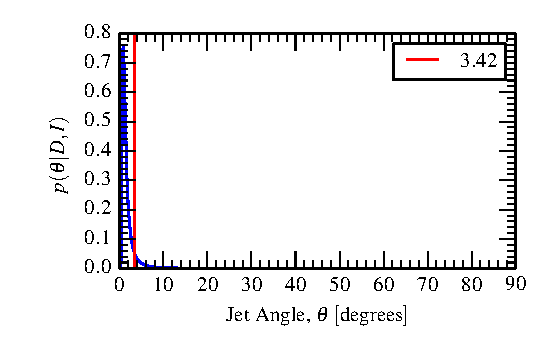
\includegraphics{jet_angle_posterior_s6UL_TEST_deltaEffPrior-1.0.eps}
\caption{$p(\epsilon|I)=\delta(\epsilon-1)$: efficiency assumed known:
$\epsilon=1$}
\end{figure}

\begin{figure}[h!]
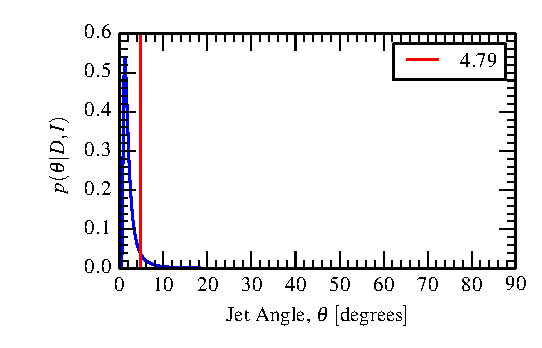
\includegraphics{jet_angle_posterior_s6UL_TEST_deltaEffPrior-0.5.eps}
\caption{$p(\epsilon|I)=\delta(\epsilon-0.5)$: efficiency assumed known:
$\epsilon=0.5$}
\end{figure}

\begin{figure}[h!]
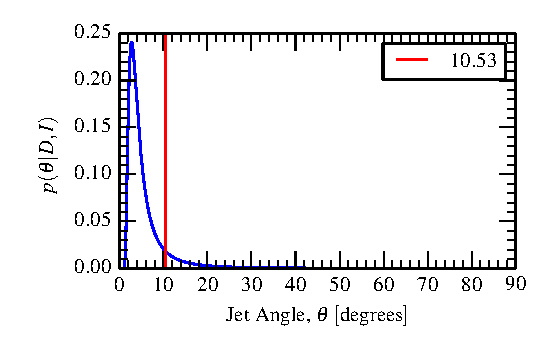
\includegraphics{jet_angle_posterior_s6UL_TEST_deltaEffPrior-0.1.eps}
\caption{$p(\epsilon|I)=\delta(\epsilon-0.1)$: efficiency assumed known:
$\epsilon=0.1$}
\end{figure}

\begin{figure}[h!]
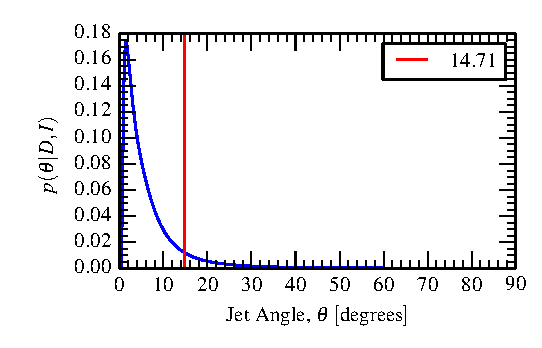
\includegraphics{jet_angle_posterior_s6UL_TEST_flatEffPrior-0.01-1.eps}
\caption{$p(\epsilon|I) \propto 1,~\epsilon \in (0,1]$. 
Here, we assume the GRB efficiency is $\epsilon \in (0,1]$, with no
preference where: the linearly uniform prior.  The reason for choosing a
non-zero lower bound is that the Jacobian determinant goes to $\inf$ as
$\epsilon \rightarrow 0$.  \textcolor{red}{James: I'm very open to suggestions
here as it's not clear to me that this is expected.  In practice, $\epsilon \in
[0.01,1]$}.}
\end{figure}

\begin{figure}[h!]
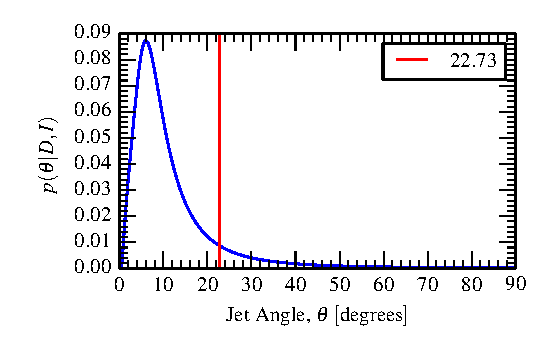
\includegraphics{jet_angle_posterior_s6UL_TEST_logEffPrior-0.01-1.eps}
\caption{$p(\epsilon|I) \propto 1/\epsilon,~\epsilon \in (0,1]$
Now assume the GRB efficiency is $\epsilon \in (0,1]$, with a log-uniform
prior (commonly but incorrectly referred to as the Jeffrey's prior).  Here, the
requirement of a non-zero lower bound is imposed by the normalisation for this
prior.
}
\end{figure}

\begin{figure}[h!]
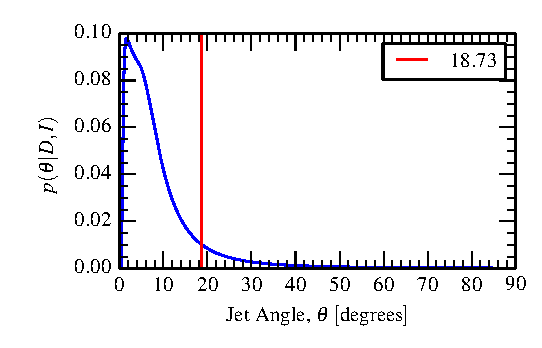
\includegraphics{jet_angle_posterior_s6UL_TEST_bernoEffPrior.eps}
\caption{$p(\epsilon|I) = \beta(1/2,1/2),~\epsilon \in (0,1)$.  Here, we use a
Beta distribution with shape and scale parameters of 1/2.  That prior has a
slightly surprising shape with a minimum at $\epsilon=0.5$ and shoots off to
$\infty$ as $\epsilon\rightarrow 0,1$.  It seems \emph{this} is, in fact, the
Jeffrey's prior for a Bernoulli trial (if we say a toin coss = BNS
$\rightarrow$GRB). See
\href{http://en.wikipedia.org/wiki/Jeffreys_prior}{http://en.wikipedia.org/wiki/Jeffreys\_prior}
}
\end{figure}

\begin{figure}[h!]
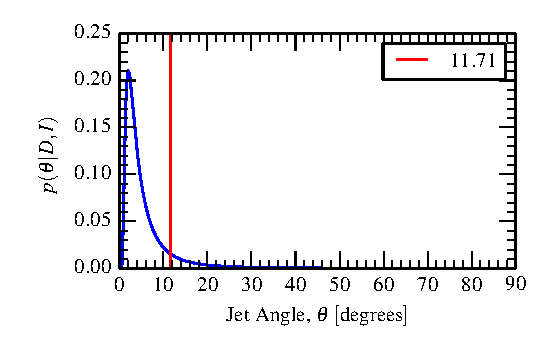
\includegraphics{jet_angle_posterior_s6UL_TEST_betaEffPrior-2-5.eps}
\caption{$p(\epsilon|I) = \beta(2,5),~\epsilon \in (0,1)$.  The GRB efficiency
prior is, this time, a $\beta$ distribution with shape and scale parameters 2
and 5, respectively.  This is now completely ad hoc but yields a maximum (in the
prior) around $\epsilon=0.2$ and goes to 0 as $\epsilon \rightarrow 0,1$.  So
it's a nice example of an asymmetric distribution with quite sensible (and
presumably tuneable) behaviour.}
\end{figure}

\begin{figure}[h!]
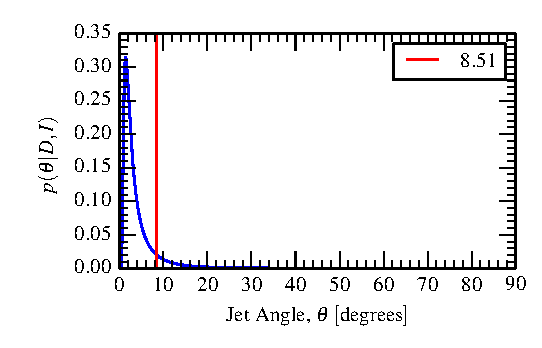
\includegraphics{jet_angle_posterior_s6UL_TEST_betaEffPrior-2-2.eps}
\caption{$p(\epsilon|I) = \beta(2,2),~\epsilon \in (0,1)$.  Finally, we have for
the GRB efficiency prior a $\beta$ distribution with shape and scale parameters 2
and 2, respectively.  Again, this is ad hoc but symmetric about $\epsilon=0.5$
with a cosine-like shape.}
\end{figure}

\bibliography{grb_beams}

\end{document}
